\documentclass{extbook}[14pt]
\usepackage{multicol, enumerate, enumitem, hyperref, color, soul, setspace, parskip, fancyhdr, amssymb, amsthm, amsmath, latexsym, units, mathtools}
\everymath{\displaystyle}
\usepackage[headsep=0.5cm,headheight=0cm, left=1 in,right= 1 in,top= 1 in,bottom= 1 in]{geometry}
\usepackage{dashrule}  % Package to use the command below to create lines between items
\newcommand{\litem}[1]{\item #1

\rule{\textwidth}{0.4pt}}
\pagestyle{fancy}
\lhead{}
\chead{Answer Key for Progress Quiz 7 Version B}
\rhead{}
\lfoot{3510-5252}
\cfoot{}
\rfoot{Summer C 2021}
\begin{document}
\textbf{This key should allow you to understand why you choose the option you did (beyond just getting a question right or wrong). \href{https://xronos.clas.ufl.edu/mac1105spring2020/courseDescriptionAndMisc/Exams/LearningFromResults}{More instructions on how to use this key can be found here}.}

\textbf{If you have a suggestion to make the keys better, \href{https://forms.gle/CZkbZmPbC9XALEE88}{please fill out the short survey here}.}

\textit{Note: This key is auto-generated and may contain issues and/or errors. The keys are reviewed after each exam to ensure grading is done accurately. If there are issues (like duplicate options), they are noted in the offline gradebook. The keys are a work-in-progress to give students as many resources to improve as possible.}

\rule{\textwidth}{0.4pt}

\begin{enumerate}\litem{
Construct the lowest-degree polynomial given the zeros below. Then, choose the intervals that contain the coefficients of the polynomial in the form $ax^3+bx^2+cx+d$.
\[ \frac{5}{3}, \frac{-1}{4}, \text{ and } \frac{-5}{2} \]The solution is \( 24x^{3} +26 x^{2} -95 x -25 \), which is option D.\begin{enumerate}[label=\Alph*.]
\item \( a \in [23, 25], b \in [-28, -20], c \in [-98, -94], \text{ and } d \in [21, 27] \)

$24x^{3} -26 x^{2} -95 x + 25$, which corresponds to multiplying out $(3x + 5)(4x -1)(2x -5)$.
\item \( a \in [23, 25], b \in [106, 107], c \in [123, 131], \text{ and } d \in [21, 27] \)

$24x^{3} +106 x^{2} +125 x + 25$, which corresponds to multiplying out $(3x + 5)(4x + 1)(2x + 5)$.
\item \( a \in [23, 25], b \in [26, 29], c \in [-98, -94], \text{ and } d \in [21, 27] \)

$24x^{3} +26 x^{2} -95 x + 25$, which corresponds to multiplying everything correctly except the constant term.
\item \( a \in [23, 25], b \in [26, 29], c \in [-98, -94], \text{ and } d \in [-26, -21] \)

* $24x^{3} +26 x^{2} -95 x -25$, which is the correct option.
\item \( a \in [23, 25], b \in [90, 99], c \in [74, 78], \text{ and } d \in [-26, -21] \)

$24x^{3} +94 x^{2} +75 x -25$, which corresponds to multiplying out $(3x + 5)(4x -1)(2x + 5)$.
\end{enumerate}

\textbf{General Comment:} To construct the lowest-degree polynomial, you want to multiply out $(3x -5)(4x + 1)(2x + 5)$
}
\litem{
Describe the zero behavior of the zero $x = -3$ of the polynomial below.
\[ f(x) = -2(x - 3)^{4}(x + 3)^{7}(x + 2)^{7}(x - 2)^{10} \]The solution is the graph below, which is option D.
    \begin{center}
        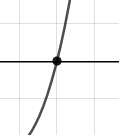
\includegraphics[width=0.3\textwidth]{../Figures/polyZeroBehaviorCopyDB.png}
    \end{center}\begin{enumerate}[label=\Alph*.]
\begin{multicols}{2}
\item 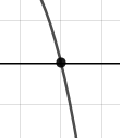
\includegraphics[width = 0.3\textwidth]{../Figures/polyZeroBehaviorCopyAB.png}
\item 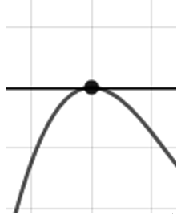
\includegraphics[width = 0.3\textwidth]{../Figures/polyZeroBehaviorCopyBB.png}
\item 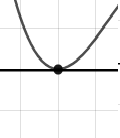
\includegraphics[width = 0.3\textwidth]{../Figures/polyZeroBehaviorCopyCB.png}
\item 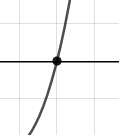
\includegraphics[width = 0.3\textwidth]{../Figures/polyZeroBehaviorCopyDB.png}
\end{multicols}\item None of the above.\end{enumerate}
\textbf{General Comment:} You will need to sketch the entire graph, then zoom in on the zero the question asks about.
}
\litem{
Which of the following equations \textit{could} be of the graph presented below?

\begin{center}
    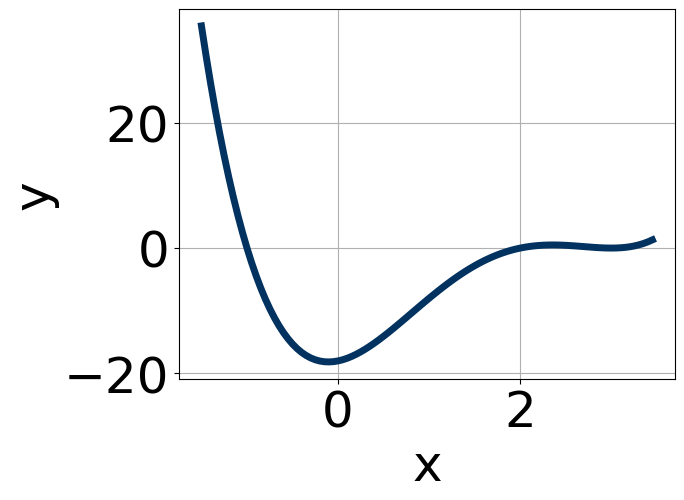
\includegraphics[width=0.5\textwidth]{../Figures/polyGraphToFunctionCopyB.png}
\end{center}


The solution is \( 5(x - 3)^{10} (x - 2)^{11} (x + 1)^{11} \), which is option B.\begin{enumerate}[label=\Alph*.]
\item \( 18(x - 3)^{4} (x - 2)^{10} (x + 1)^{11} \)

The factor $(x - 2)$ should have an odd power.
\item \( 5(x - 3)^{10} (x - 2)^{11} (x + 1)^{11} \)

* This is the correct option.
\item \( -14(x - 3)^{10} (x - 2)^{11} (x + 1)^{4} \)

The factor $(x + 1)$ should have an odd power and the leading coefficient should be the opposite sign.
\item \( 18(x - 3)^{7} (x - 2)^{4} (x + 1)^{7} \)

The factor $3$ should have an even power and the factor $2$ should have an odd power.
\item \( -10(x - 3)^{4} (x - 2)^{9} (x + 1)^{11} \)

This corresponds to the leading coefficient being the opposite value than it should be.
\end{enumerate}

\textbf{General Comment:} General Comments: Draw the x-axis to determine which zeros are touching (and so have even multiplicity) or cross (and have odd multiplicity).
}
\litem{
Construct the lowest-degree polynomial given the zeros below. Then, choose the intervals that contain the coefficients of the polynomial in the form $x^3+bx^2+cx+d$.
\[ -3 - 4 i \text{ and } -3 \]The solution is \( x^{3} +9 x^{2} +43 x + 75 \), which is option C.\begin{enumerate}[label=\Alph*.]
\item \( b \in [-3, 3], c \in [6.2, 9.3], \text{ and } d \in [12, 14] \)

$x^{3} + x^{2} +7 x + 12$, which corresponds to multiplying out $(x + 4)(x + 3)$.
\item \( b \in [-12, -8], c \in [42, 47.2], \text{ and } d \in [-75, -74] \)

$x^{3} -9 x^{2} +43 x -75$, which corresponds to multiplying out $(x-(-3 - 4 i))(x-(-3 + 4 i))(x -3)$.
\item \( b \in [9, 13], c \in [42, 47.2], \text{ and } d \in [72, 82] \)

* $x^{3} +9 x^{2} +43 x + 75$, which is the correct option.
\item \( b \in [-3, 3], c \in [2.5, 6.7], \text{ and } d \in [5, 11] \)

$x^{3} + x^{2} +6 x + 9$, which corresponds to multiplying out $(x + 3)(x + 3)$.
\item \( \text{None of the above.} \)

This corresponds to making an unanticipated error or not understanding how to use nonreal complex numbers to create the lowest-degree polynomial. If you chose this and are not sure what you did wrong, please contact the coordinator for help.
\end{enumerate}

\textbf{General Comment:} Remember that the conjugate of $a+bi$ is $a-bi$. Since these zeros always come in pairs, we need to multiply out $(x-(-3 - 4 i))(x-(-3 + 4 i))(x-(-3))$.
}
\litem{
Which of the following equations \textit{could} be of the graph presented below?

\begin{center}
    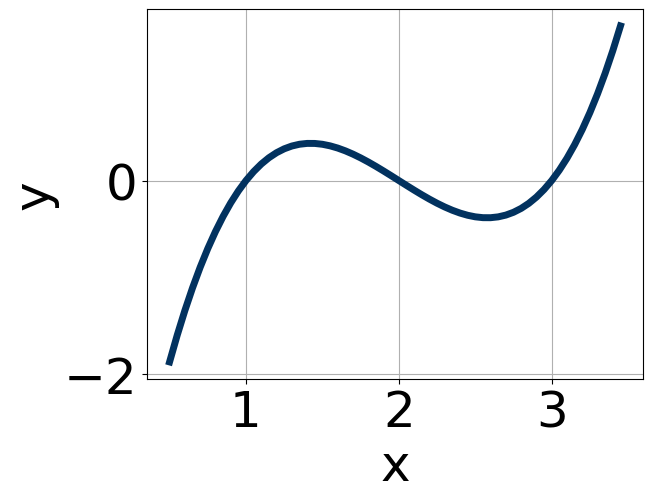
\includegraphics[width=0.5\textwidth]{../Figures/polyGraphToFunctionB.png}
\end{center}


The solution is \( 4(x - 1)^{7} (x - 2)^{5} (x - 3)^{9} \), which is option D.\begin{enumerate}[label=\Alph*.]
\item \( -20(x - 1)^{8} (x - 2)^{9} (x - 3)^{5} \)

The factor $(x - 1)$ should have an odd power and the leading coefficient should be the opposite sign.
\item \( 20(x - 1)^{8} (x - 2)^{5} (x - 3)^{7} \)

The factor $1$ should have been an odd power.
\item \( -5(x - 1)^{11} (x - 2)^{11} (x - 3)^{5} \)

This corresponds to the leading coefficient being the opposite value than it should be.
\item \( 4(x - 1)^{7} (x - 2)^{5} (x - 3)^{9} \)

* This is the correct option.
\item \( 7(x - 1)^{8} (x - 2)^{6} (x - 3)^{7} \)

The factors $1$ and $2$ have have been odd power.
\end{enumerate}

\textbf{General Comment:} General Comments: Draw the x-axis to determine which zeros are touching (and so have even multiplicity) or cross (and have odd multiplicity).
}
\litem{
Describe the zero behavior of the zero $x = 5$ of the polynomial below.
\[ f(x) = 4(x - 2)^{6}(x + 2)^{3}(x - 5)^{7}(x + 5)^{2} \]The solution is the graph below, which is option D.
    \begin{center}
        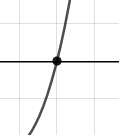
\includegraphics[width=0.3\textwidth]{../Figures/polyZeroBehaviorDB.png}
    \end{center}\begin{enumerate}[label=\Alph*.]
\begin{multicols}{2}
\item 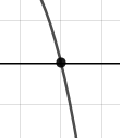
\includegraphics[width = 0.3\textwidth]{../Figures/polyZeroBehaviorAB.png}
\item 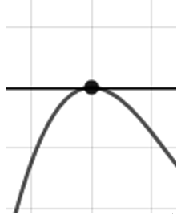
\includegraphics[width = 0.3\textwidth]{../Figures/polyZeroBehaviorBB.png}
\item 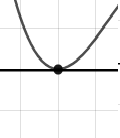
\includegraphics[width = 0.3\textwidth]{../Figures/polyZeroBehaviorCB.png}
\item 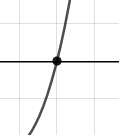
\includegraphics[width = 0.3\textwidth]{../Figures/polyZeroBehaviorDB.png}
\end{multicols}\item None of the above.\end{enumerate}
\textbf{General Comment:} You will need to sketch the entire graph, then zoom in on the zero the question asks about.
}
\litem{
Describe the end behavior of the polynomial below.
\[ f(x) = -2(x + 2)^{3}(x - 2)^{8}(x - 9)^{4}(x + 9)^{6} \]The solution is the graph below, which is option A.
    \begin{center}
        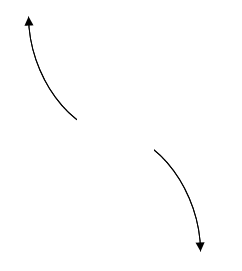
\includegraphics[width=0.3\textwidth]{../Figures/polyEndBehaviorAB.png}
    \end{center}\begin{enumerate}[label=\Alph*.]
\begin{multicols}{2}
\item 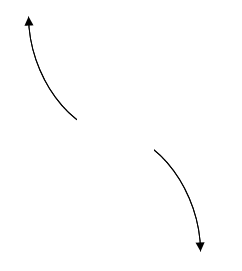
\includegraphics[width = 0.3\textwidth]{../Figures/polyEndBehaviorAB.png}
\item 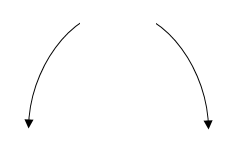
\includegraphics[width = 0.3\textwidth]{../Figures/polyEndBehaviorBB.png}
\item 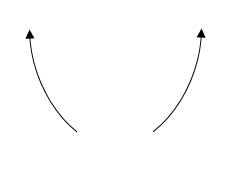
\includegraphics[width = 0.3\textwidth]{../Figures/polyEndBehaviorCB.png}
\item 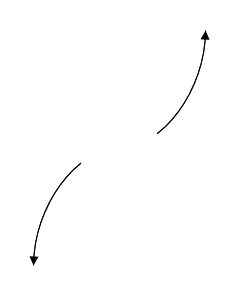
\includegraphics[width = 0.3\textwidth]{../Figures/polyEndBehaviorDB.png}
\end{multicols}\item None of the above.\end{enumerate}
\textbf{General Comment:} Remember that end behavior is determined by the leading coefficient AND whether the \textbf{sum} of the multiplicities is positive or negative.
}
\litem{
Describe the end behavior of the polynomial below.
\[ f(x) = -4(x - 5)^{5}(x + 5)^{8}(x - 4)^{5}(x + 4)^{5} \]The solution is the graph below, which is option A.
    \begin{center}
        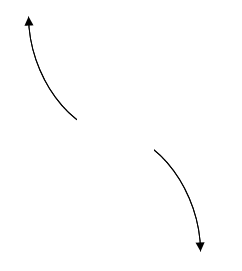
\includegraphics[width=0.3\textwidth]{../Figures/polyEndBehaviorCopyAB.png}
    \end{center}\begin{enumerate}[label=\Alph*.]
\begin{multicols}{2}
\item 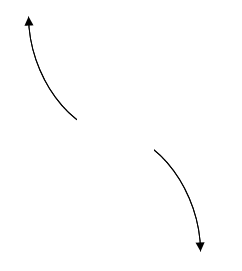
\includegraphics[width = 0.3\textwidth]{../Figures/polyEndBehaviorCopyAB.png}
\item 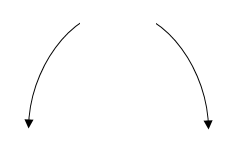
\includegraphics[width = 0.3\textwidth]{../Figures/polyEndBehaviorCopyBB.png}
\item 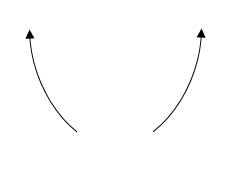
\includegraphics[width = 0.3\textwidth]{../Figures/polyEndBehaviorCopyCB.png}
\item 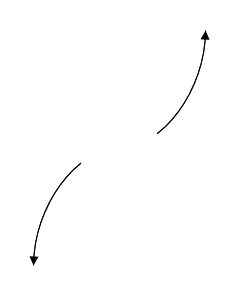
\includegraphics[width = 0.3\textwidth]{../Figures/polyEndBehaviorCopyDB.png}
\end{multicols}\item None of the above.\end{enumerate}
\textbf{General Comment:} Remember that end behavior is determined by the leading coefficient AND whether the \textbf{sum} of the multiplicities is positive or negative.
}
\litem{
Construct the lowest-degree polynomial given the zeros below. Then, choose the intervals that contain the coefficients of the polynomial in the form $ax^3+bx^2+cx+d$.
\[ \frac{4}{3}, \frac{1}{4}, \text{ and } 1 \]The solution is \( 12x^{3} -31 x^{2} +23 x -4 \), which is option D.\begin{enumerate}[label=\Alph*.]
\item \( a \in [11, 21], b \in [-0.6, 2.1], c \in [-19.5, -16.4], \text{ and } d \in [2, 6] \)

$12x^{3} + x^{2} -17 x + 4$, which corresponds to multiplying out $(3x + 4)(4x -1)(x -1)$.
\item \( a \in [11, 21], b \in [1.5, 8.2], c \in [-16, -14.6], \text{ and } d \in [-6, 0] \)

$12x^{3} +7 x^{2} -15 x -4$, which corresponds to multiplying out $(3x + 4)(4x + 1)(x -1)$.
\item \( a \in [11, 21], b \in [30.9, 32.5], c \in [20.5, 27.3], \text{ and } d \in [2, 6] \)

$12x^{3} +31 x^{2} +23 x + 4$, which corresponds to multiplying out $(3x + 4)(4x + 1)(x + 1)$.
\item \( a \in [11, 21], b \in [-32.9, -28.5], c \in [20.5, 27.3], \text{ and } d \in [-6, 0] \)

* $12x^{3} -31 x^{2} +23 x -4$, which is the correct option.
\item \( a \in [11, 21], b \in [-32.9, -28.5], c \in [20.5, 27.3], \text{ and } d \in [2, 6] \)

$12x^{3} -31 x^{2} +23 x + 4$, which corresponds to multiplying everything correctly except the constant term.
\end{enumerate}

\textbf{General Comment:} To construct the lowest-degree polynomial, you want to multiply out $(3x -4)(4x -1)(x -1)$
}
\litem{
Construct the lowest-degree polynomial given the zeros below. Then, choose the intervals that contain the coefficients of the polynomial in the form $x^3+bx^2+cx+d$.
\[ -2 + 3 i \text{ and } -1 \]The solution is \( x^{3} +5 x^{2} +17 x + 13 \), which is option D.\begin{enumerate}[label=\Alph*.]
\item \( b \in [0.1, 3.9], c \in [-7, 0], \text{ and } d \in [-5.5, -1.1] \)

$x^{3} + x^{2} -2 x -3$, which corresponds to multiplying out $(x -3)(x + 1)$.
\item \( b \in [-10.8, -3], c \in [12, 26], \text{ and } d \in [-14.5, -9.4] \)

$x^{3} -5 x^{2} +17 x -13$, which corresponds to multiplying out $(x-(-2 + 3 i))(x-(-2 - 3 i))(x -1)$.
\item \( b \in [0.1, 3.9], c \in [2, 8], \text{ and } d \in [0.4, 3.8] \)

$x^{3} + x^{2} +3 x + 2$, which corresponds to multiplying out $(x + 2)(x + 1)$.
\item \( b \in [2.5, 6.7], c \in [12, 26], \text{ and } d \in [12.3, 16.1] \)

* $x^{3} +5 x^{2} +17 x + 13$, which is the correct option.
\item \( \text{None of the above.} \)

This corresponds to making an unanticipated error or not understanding how to use nonreal complex numbers to create the lowest-degree polynomial. If you chose this and are not sure what you did wrong, please contact the coordinator for help.
\end{enumerate}

\textbf{General Comment:} Remember that the conjugate of $a+bi$ is $a-bi$. Since these zeros always come in pairs, we need to multiply out $(x-(-2 + 3 i))(x-(-2 - 3 i))(x-(-1))$.
}
\end{enumerate}

\end{document}